\section{Наклонная Волоконная Брэгговская Решётка}
Чтобы понять физику наклонных волокон удобно рассмотреть спектры коэффицентов 
пропускания и отражения пары идентичных решёток наклонённые относительно друг друга на $ 10 $ градусов.
Можно выделить два важных случая: cлучай нормальной волоконной брэгговской решётки у которой только один сильный резонанс. К примеру провал в спектре пропускания соответствует условию Брэгга для периода решётки в этом волокне и тот же резонанся появляется как одиничный пик в спектре отражения. Длина волна $ \lambda_{B} $ соответсвующая брэгговскому резонансу самая большая так эффективный показатель преломления для одной моды направленной вдоль сердцевины самый большой.




\begin{figure}[h]
	\centering
	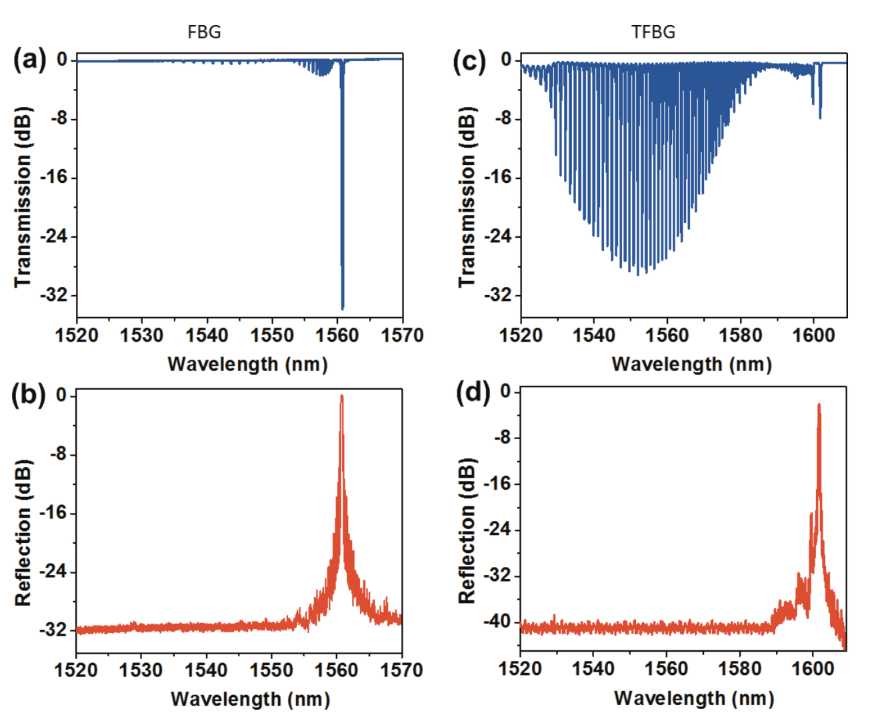
\includegraphics[width=0.7\linewidth]{screenshot001}
	\caption{}
	\label{fig:screenshot001}
\end{figure}


\begin{figure}
	\centering
	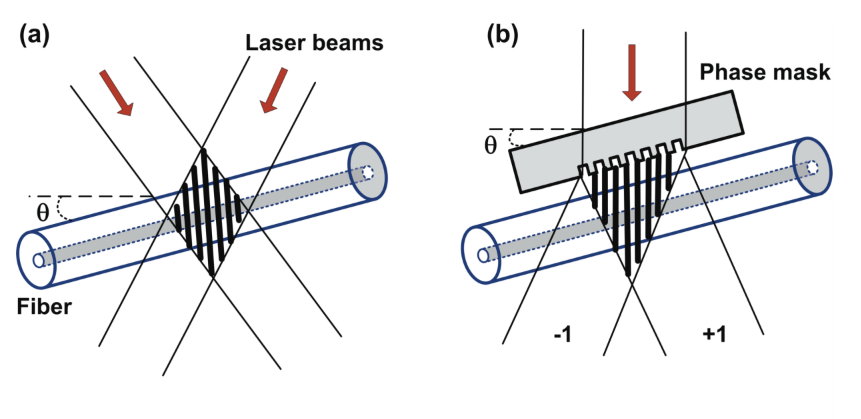
\includegraphics[width=0.7\linewidth]{screenshot005}
	\caption{}
	\label{fig:screenshot005}
\end{figure}


\begin{figure}[h]
	\centering
	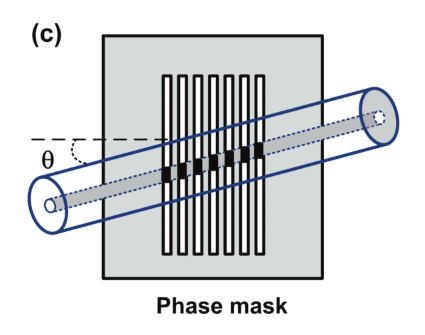
\includegraphics[width=0.4\linewidth]{screenshot004}
	\caption{}
	\label{fig:screenshot004}
\end{figure}
